\section{Desenvolvimento computacional}\label{sec:desenvolvimento}

\subsection{Arquitetura}
O GraphCube Lab é uma aplicação web em TypeScript (React~18, Vite, Three.js~\cite{threejs}, \texttt{d3-force}~\cite{bostock2011}), organizada em módulos com dependências num único sentido:
\begin{center}
\texttt{core} $\leftarrow$ \texttt{search} $\leftarrow$ \{\texttt{graph}, \texttt{experiments}\} $\leftarrow$ \{\texttt{workers}, \texttt{ui}\};\qquad \texttt{viz3d}, \texttt{vizgraph}: apenas dados.
\end{center}
O módulo \texttt{core} (permutações, geometria, notação, cubinhos, simetrias, Schreier--Sims, gerador pseudoaleatório) não depende de nenhuma biblioteca de interface. Buscas, explorações de Cayley e experimentos executam num \textit{Web Worker}, mantendo a interface responsiva e permitindo cancelamento. Os \emph{mesmos} módulos TypeScript rodam no navegador e numa interface de linha de comando em Node.js, que gera os dados deste artigo; uma etapa em Python apenas analisa os arquivos JSON resultantes. Assim, o texto descreve exatamente o software que produziu os números.

\subsection{Estruturas de dados}
\paragraph{Estados.} No nível de adesivos, um estado é um \texttt{Uint8Array} de tamanho $6n^2$. No nível de cubinhos, quatro vetores $(\sigma,x,\tau,y)$. Para a busca, usamos \emph{coordenadas}:
\begin{itemize}[nosep]
\item \cube{2}: $\mathrm{idx}=\pi\cdot729+\omega$, em que $\pi\in[0,5040)$ é a posição lexicográfica (código de Lehmer) da permutação dos 7 cantos livres e $\omega\in[0,729)$ codifica em base 3 as torções de 6 deles (a sétima é determinada pela soma). Como $|G_2|=5040\cdot729$, a codificação é uma bijeção $G_2\to[0,\num{3674160})$ (testada), o que permite armazenar todo o espaço em tabelas de acesso direto;
\item \cube{3}: as coordenadas de Kociemba~\cite{kociembaweb} --- torção (2187), inversão (2048), posições das arestas da camada E (495), permutação dos cantos (40\,320), permutação das 8 arestas U/D (40\,320) e das 4 arestas E (24).
\end{itemize}
Tabelas de movimento são calculadas aplicando a multiplicação de cubinhos a um representante de cada valor de coordenada; a consistência entre tabela e multiplicação é testada.

\paragraph{Busca.} Um espaço de busca é uma interface (\texttt{SearchSpace}) com estado inicial, objetivo, função de chave, aplicação de movimentos e regras de poda; o grafo é sempre implícito. Conjuntos de visitados usam tabelas de acesso direto quando as chaves são inteiros limitados (\cube{2}) e \texttt{Map} caso contrário. A$^*$ usa um heap binário com desempate pelo maior $g$. Cada execução devolve as mesmas métricas: nós expandidos, gerados, descobertos (distintos), pico de estados armazenados, profundidade, tempo, iterações (IDA$^*$) e, opcionalmente, um \emph{registro de eventos} (\texttt{discover}, \texttt{expand}, \texttt{bound}, \texttt{meet}, \texttt{goal}) na ordem exata da execução, truncado após um limite configurável e marcado como tal.

\paragraph{Tabelas exatas e PDBs.} A distância exata $d^*$ de todos os estados do \cube{2} é calculada por uma BFS a partir de $e$ com fila em \texttt{Int32Array} (HTM e QTM em cerca de \gclBfsTimeHTM{} e \gclBfsTimeQTM{}~ms em Node.js). As PDBs são BFS nos espaços de coordenadas projetadas. As tabelas do \cube{3} (movimentos e podas das duas fases e das PDBs) são construídas em cerca de \gclTwoPhaseTables{}~ms.

\begin{algorithm}[t]
\caption{IDA$^*$ com poda canônica, como implementado (\texttt{search/algorithms.ts}).}\label{alg:ida}
\begin{algorithmic}[1]
\Require espaço $(s_0,\mathrm{apply},\mathrm{goal})$, heurística $h$ admissível
\Ensure palavra mínima de $s_0$ ao objetivo (ou falha por limite)
\State $\theta\gets h(s_0)$
\Loop
  \State $t\gets\Call{DFS}{s_0,0,\theta,\bot}$
  \If{$t=\textsc{achou}$} \Return caminho \EndIf
  \If{$t=\infty$ ou limite de nós/tempo} \Return falha \EndIf
  \State $\theta\gets t$ \Comment{menor $f$ que excedeu o limiar}
\EndLoop
\Function{DFS}{$s,g,\theta,\ell$}
  \State $f\gets g+h(s)$; \textbf{if} $f>\theta$ \textbf{return} $f$
  \State \textbf{if} $s$ é objetivo \textbf{return} \textsc{achou}
  \State $\mu\gets\infty$
  \For{$m\in\mathrm{canonicalAfter}(\ell)$}
     \State $t\gets\Call{DFS}{\mathrm{apply}(s,m),g+1,\theta,m}$
     \State \textbf{if} $t=\textsc{achou}$ \textbf{return} \textsc{achou}; $\mu\gets\min(\mu,t)$
  \EndFor
  \State \Return $\mu$
\EndFunction
\end{algorithmic}
\end{algorithm}

\subsection{Método de duas fases}
Implementamos o algoritmo de Kociemba~\cite{kociemba1992,kociembaweb}. A fase~1 é um IDA$^*$ em $G$ até o subgrupo $H=\langle\mv U,\mv D,\mv{R2},\mv{L2},\mv{F2},\mv{B2}\rangle$ (torção, inversão e posição das arestas E corretas) e a fase~2 é um IDA$^*$ em $H$ até $e$, com heurísticas
\begin{equation*}
h_1=\max\bigl(P[\text{torção},\text{E}],\,P[\text{inversão},\text{E}]\bigr),\qquad
h_2=\max\bigl(P[\text{cantos},\pi_E],\,P[\pi_{UD},\pi_E]\bigr).
\end{equation*} Soluções da fase~1 são enumeradas por comprimento crescente (descartando as que terminam com movimento de $H$, que seriam redundantes) e cada uma é completada pela fase~2 limitada pela melhor solução total encontrada, até atingir um comprimento-alvo ou um limite de tempo. O resultado é sempre uma solução \emph{válida} (verificada nos testes aplicando-a ao estado), mas \emph{não necessariamente mínima}: a decomposição $G\to H\to e$ exclui caminhos que deixam $H$ após entrar nele. Verificamos que $|H|=8!\cdot8!\cdot4!/2=\num{19508428800}$ por Schreier--Sims\ver.

\subsection{Visualização}
\paragraph{Cubo 3D.} O renderizador Three.js não guarda estado lógico: ele recebe o estado e a fila de movimentos. Para animar um giro, agrupa os cubinhos da camada num pivô, interpola a rotação (curva cúbica \textit{ease-in-out}) e, ao final, devolve todos os cubinhos à posição de origem e \emph{recolore} os adesivos a partir do estado lógico. Assim não há acúmulo de erro de ponto flutuante --- defeito presente na implementação original, que identificava peças por posição com tolerância. A manipulação direta escolhe, entre as duas rotações perpendiculares à normal do adesivo tocado, a de velocidade projetada na tela mais alinhada com o arraste.

\paragraph{Grafo estrutural.} Desenhado em SVG com a construção da \cref{prop:estrutural}. O arraste ao longo de um círculo gira rigidamente os adesivos do anel; ao soltar, escolhe-se $k\in\{0,1,2,3\}$ minimizando a distância entre a posição visual do adesivo arrastado e $\sigma^k$ da sua posição, o que independe de os pontos estarem igualmente espaçados no círculo. Ao passar o mouse sobre um movimento, seus ciclos em $\Omega$ são desenhados como arcos (anel) e setas (face).

\paragraph{Grafos de estados, de Cayley e de busca.} Renderizados em \textit{canvas} com layout por forças incremental, preservando posições entre atualizações. O grafo de estados mostra o estado atual, o histórico, estados repetidos, ciclos detectados e caminhos de solução; a cor é $d^*$ exato (\cube{2}) ou o limite inferior $h_{\mathrm{PDB}}$ (\cube{3}). No modo Cayley, $|\langle S\rangle|$ é calculado por Schreier--Sims e qualquer bola desenhada é rotulada como \emph{parcial} quando não contém todo o grupo. A visualização de busca \emph{reproduz o registro de eventos real}, distinguindo expandidos, fronteira e caminho; nada é sintetizado.

\begin{figure}[t]
  \centering
  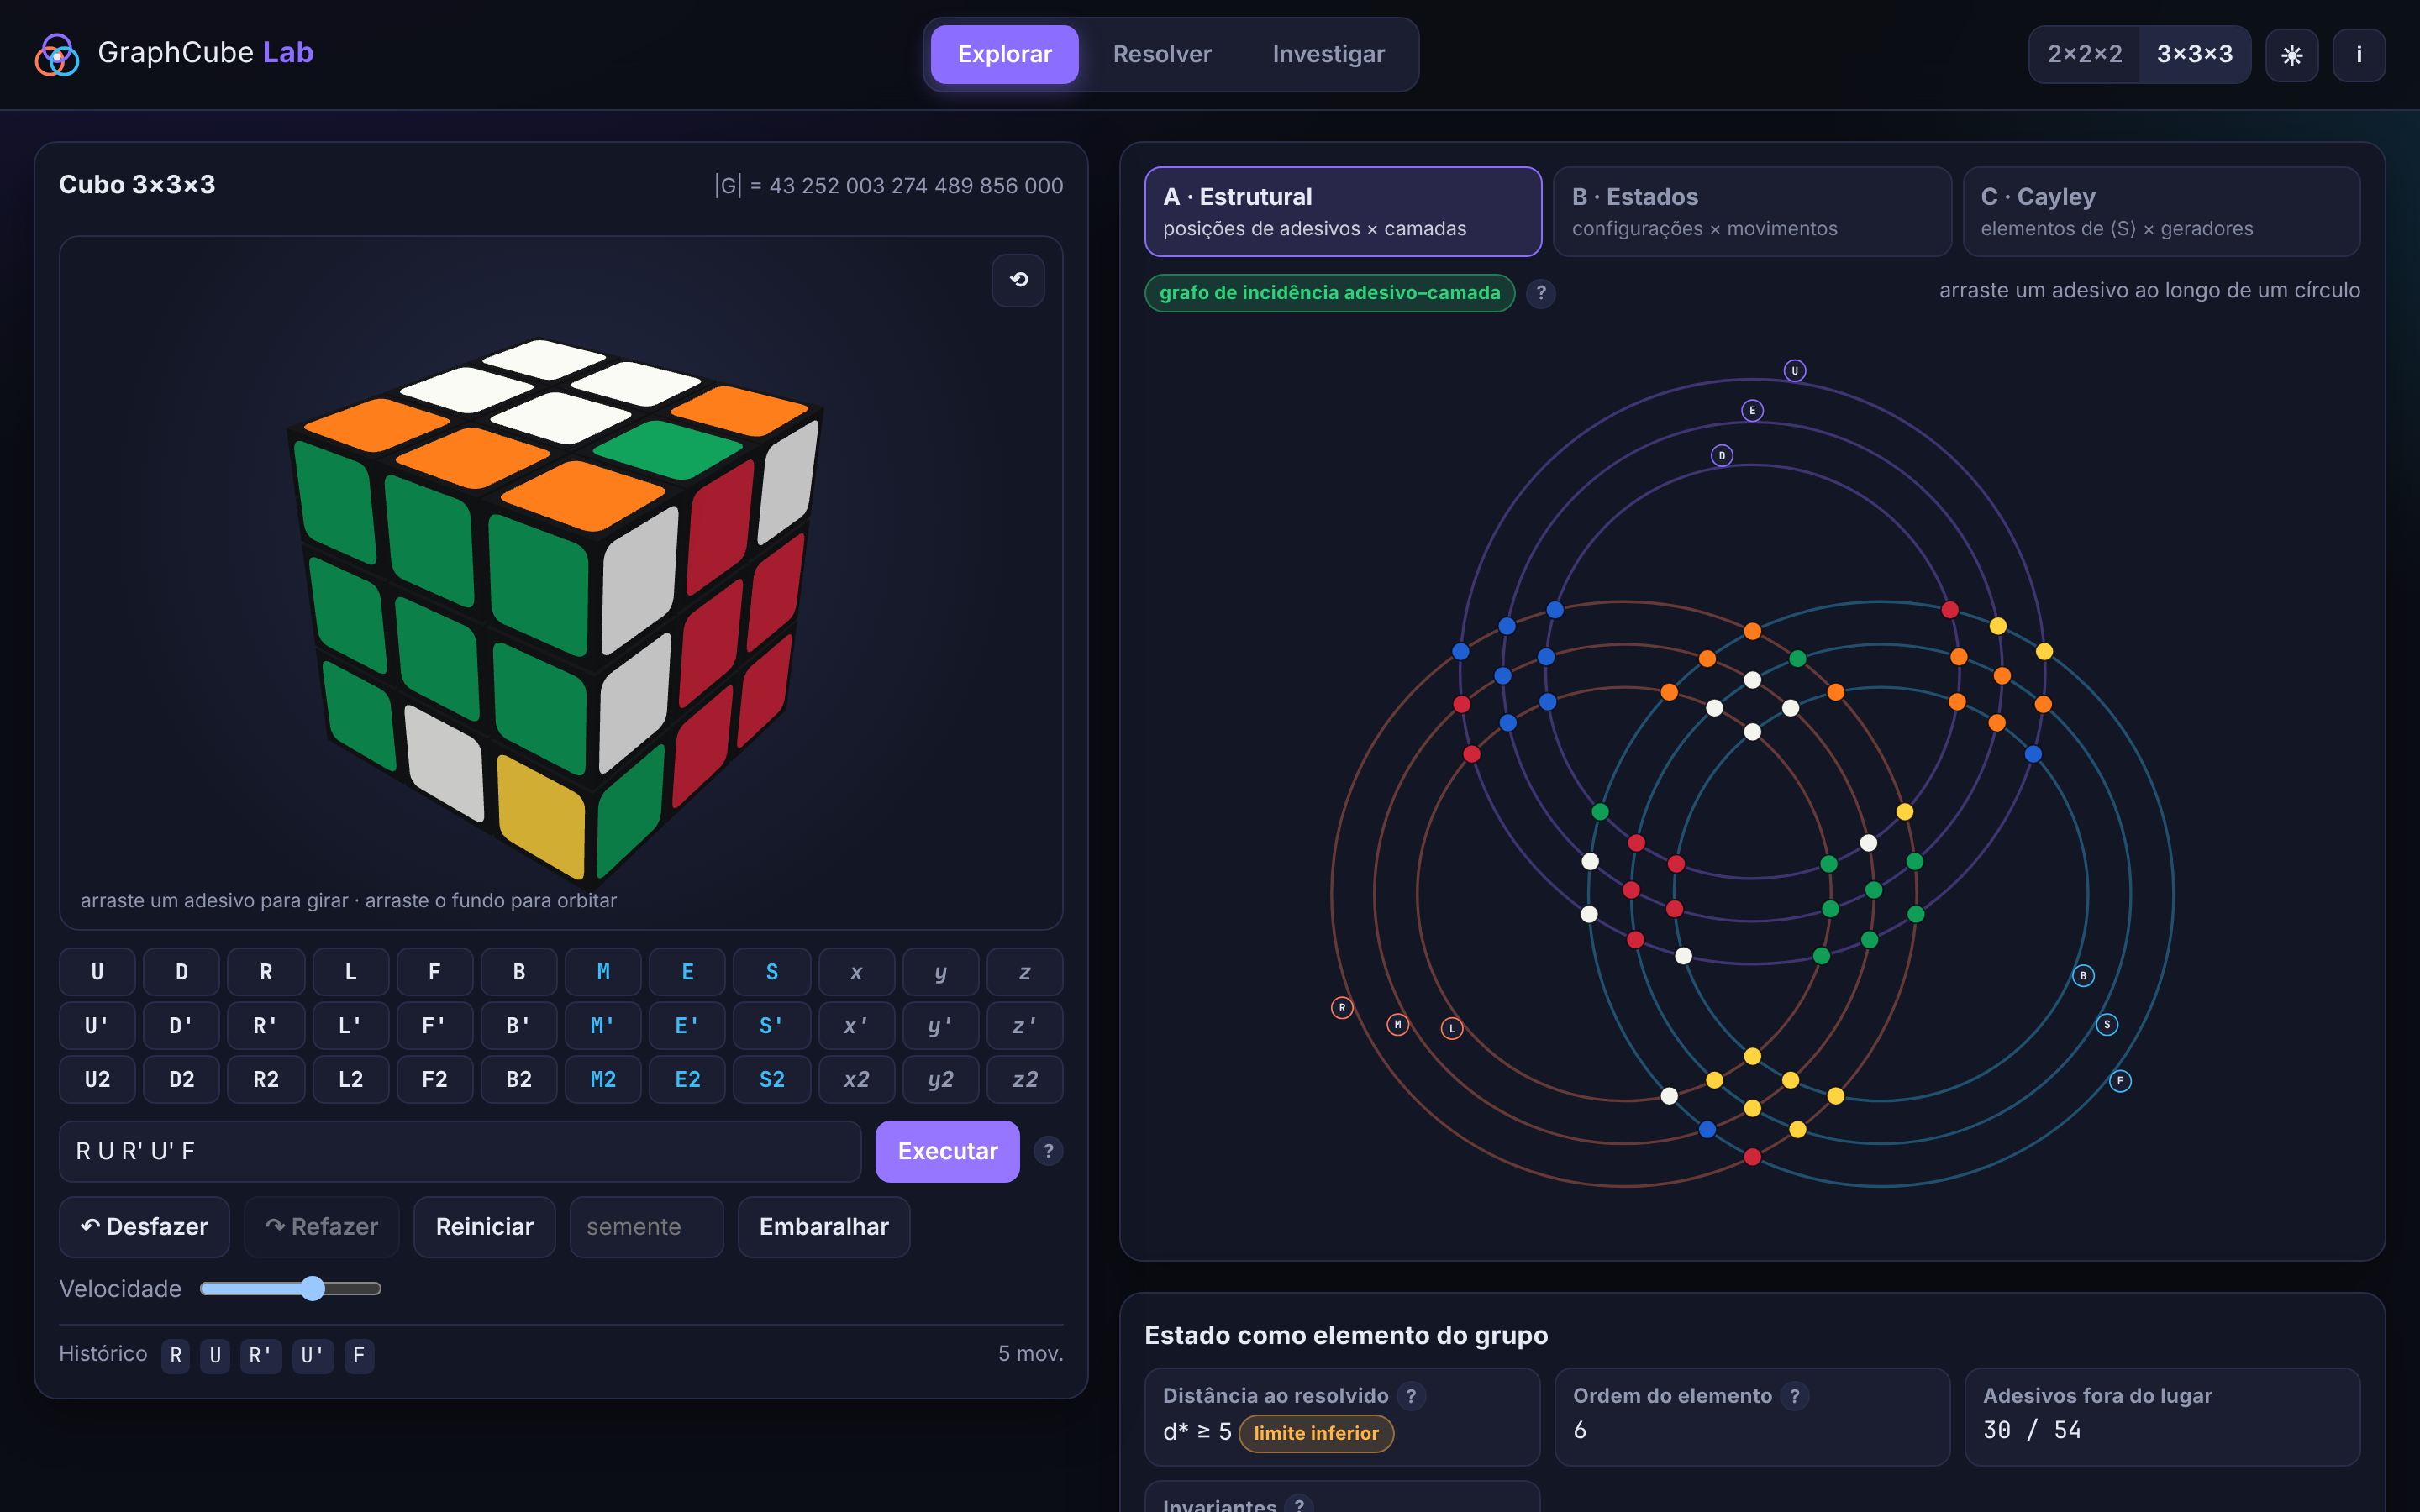
\includegraphics[width=\linewidth]{app-explorar.png}
  \caption{Modo \emph{Explorar} após \mv{R U R' U' F}: cubo 3D, grafo estrutural (posições de adesivos nas interseções dos círculos das camadas) e o estado visto como elemento do grupo (ciclos de cantos e arestas, invariantes, ordem e limite inferior para $d^*$).}
  \label{fig:interface}
\end{figure}

\begin{figure}[t]
  \centering
  \begin{subfigure}[t]{0.49\linewidth}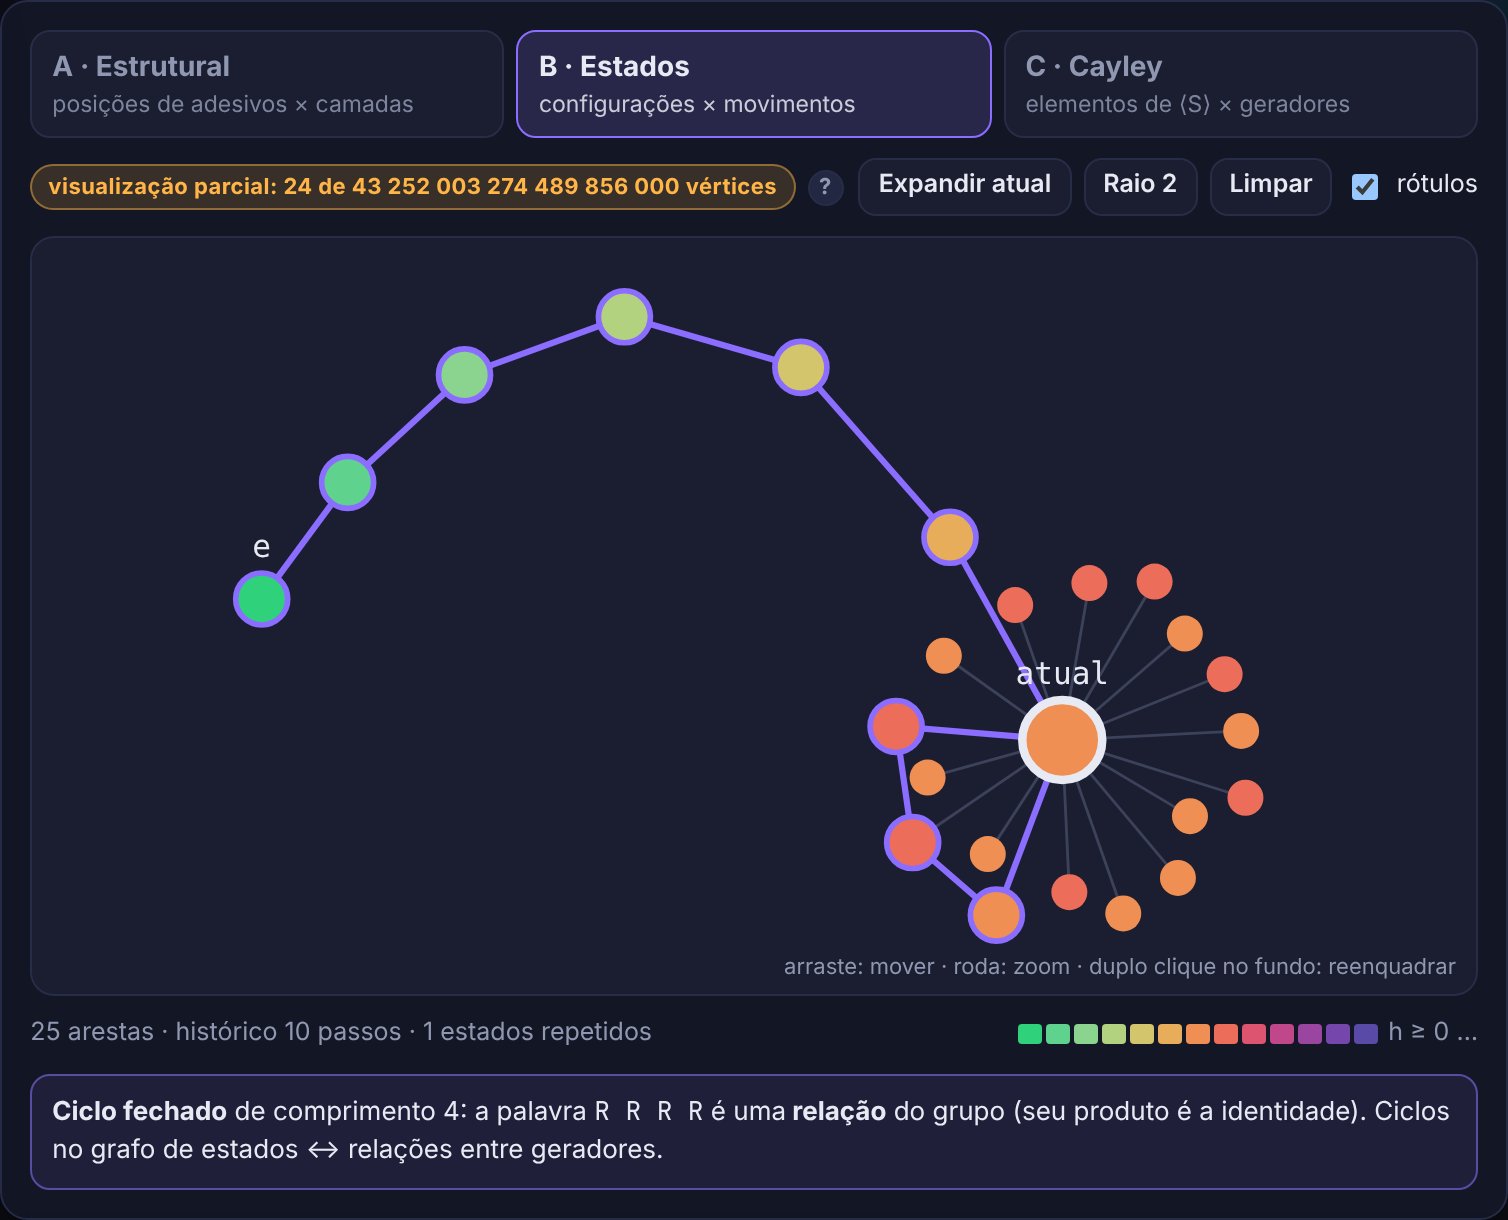
\includegraphics[width=\linewidth]{estados.png}\caption{Grafo de estados após \mv{U R R R R} e expansão local: o ciclo $\mv R^4=e$ é detectado.}\end{subfigure}\hfill
  \begin{subfigure}[t]{0.49\linewidth}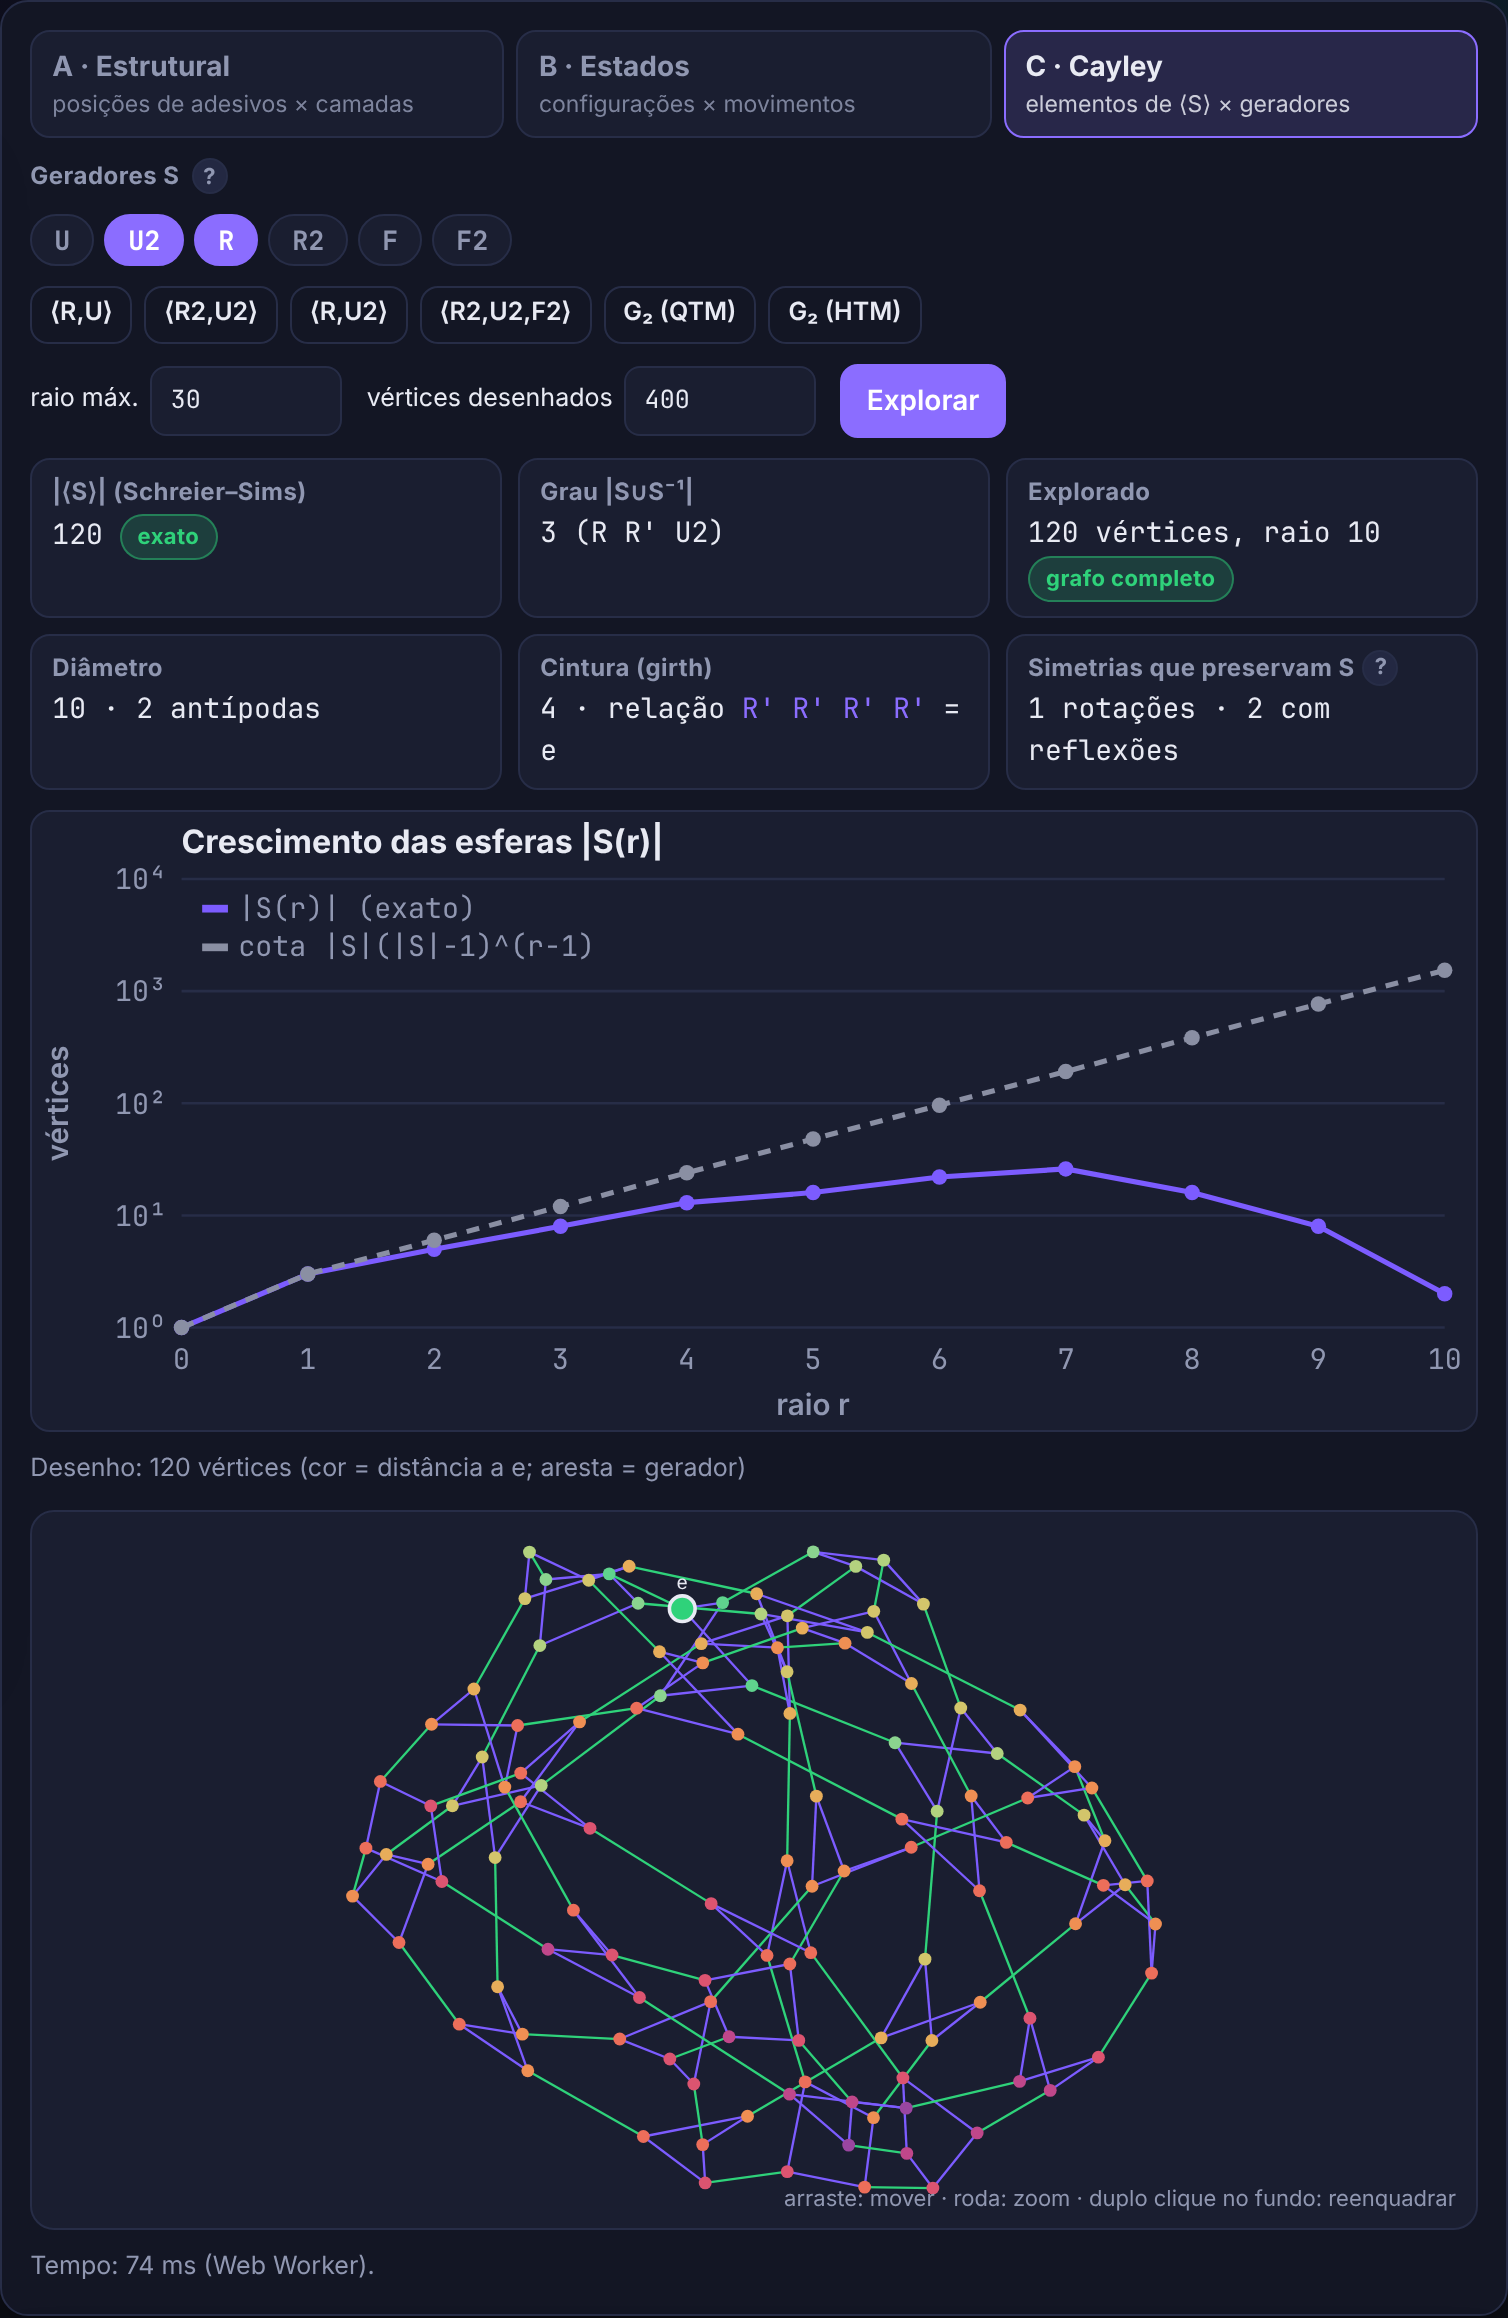
\includegraphics[width=\linewidth,trim=0 60 0 1480,clip]{cayley.png}\caption{$\Cay(\langle\mv R,\mv{U2}\rangle)$ no \cube{2}: grupo de ordem 120, diâmetro 10, cintura 4.}\end{subfigure}
  \caption{Representações (B) e (C) na interface. Os rótulos indicam quando a visualização é parcial.}
  \label{fig:grafos}
\end{figure}

\subsection{Testes}
A suíte automatizada (Vitest) tem 55 testes, organizados em: axiomas de grupo em permutações aleatórias; geometria (54 adesivos, tabelas de Kociemba, cadeias de facelets conhecidas para \mv U, \mv R, \mv F); identidade, inversos, composição e homomorfismo de palavras; ordens clássicas; comutadores, conjugados e relações entre fatias e rotações; bijeção e homomorfismo adesivos$\leftrightarrow$cubinhos; invariantes de legalidade; simetrias e referencial canônico; ordens de grupos por Schreier--Sims; distribuição de distâncias do \cube{2}; admissibilidade e consistência de todas as heurísticas em amostras; otimalidade de BFS, bidirecional, A$^*$ e IDA$^*$ contra a tabela exata; fidelidade do registro de eventos; coordenadas e tabelas de Kociemba; validade das soluções de duas fases; geometria do diagrama estrutural; propriedades de grafos de Cayley; e detecção de ciclos no grafo de estados.
